\section{Mô hình hóa bài toán}
\label{sec:model}

\subsection{Phát biểu bài toán và quy tắc Bloxorz}

Trong Bloxorz, người chơi lăn khối hộp $1\times1\times2$ trên một bàn chơi
hữu hạn để đưa khối từ ô Start tới ô Goal~\cite{coolmathbloxorz}. Màn chơi
chỉ hoàn thành khi khối đứng thẳng trên Goal; khối nằm ngang hoặc nằm dọc qua
Goal chưa thỏa điều kiện đích. Ngoài Floor và Void, phiên bản của nhóm hỗ trợ
Fragile, Bridge, Soft Switch, Heavy Switch và Split Switch theo yêu cầu đề
bài~\cite{projectspec2026}.

Trò chơi có tính xác định và quan sát đầy đủ: ở mỗi thời điểm, lưới và trạng
thái hiện tại của các cầu đều được biết; từ một trạng thái và hành động hợp lệ,
kết quả được xác định duy nhất. Ta tách dữ liệu thành hai phần:

\begin{itemize}
    \item \textbf{Dữ liệu tĩnh của màn chơi}: lưới, Start, Goal, danh sách cầu,
    trạng thái mở ban đầu, công tắc và tác động của từng công tắc. Các dữ liệu này
    được xác định trước và không thay đổi trong khi tìm kiếm.
    \item \textbf{Trạng thái động}: tư thế/vị trí của khối và trạng thái mở--đóng
    của các cầu. Đây là phần phải nằm trong mỗi trạng thái tìm kiếm.
\end{itemize}

Gọi $R,C$ lần lượt là số hàng và số cột. Một màn chơi được mô tả bởi
\begin{equation}
L=(\Gamma,p_0,g,\mathcal{B},\mathcal{W}),
\end{equation}
trong đó $\Gamma$ là lưới $R\times C$, $p_0$ là Start, $g$ là Goal,
$\mathcal{B}$ là tập cầu và $\mathcal{W}$ là tập công tắc.

\begin{table}[H]
\centering
\caption{Các loại ô cơ bản trong lưới của màn chơi}
\label{tab:grid-symbols}
\small
\begin{tabular}{@{}cll@{}}
\toprule
\textbf{Ký hiệu} & \textbf{Loại ô} & \textbf{Ý nghĩa} \\
\midrule
\texttt{.} & Floor & Ô sàn thông thường \\
\texttt{\#} & Void & Không có sàn; có thể được một cầu phủ lên \\
\texttt{S} & Start & Vị trí ban đầu của khối đứng \\
\texttt{G} & Goal & Đích; chỉ khối nguyên đứng mới hoàn thành màn chơi \\
\texttt{F} & Fragile & Không chịu được khối nguyên ở tư thế đứng \\
\bottomrule
\end{tabular}
\end{table}

\subsection{Biểu diễn không gian trạng thái}

Một trạng thái đầy đủ được biểu diễn bởi
\begin{equation}
s=(b,m),
\end{equation}
trong đó $b$ mô tả khối và $m$ là mặt nạ bit lưu trạng thái các cầu. Thành phần
$b$ phải ghi tư thế khi khối nguyên, hoặc chỉ số khối lập phương đang được điều
khiển khi khối tách. Thiếu thông tin này, trạng thái không xác định được nước
đi kế tiếp.

\subsubsection{Khối nguyên}

Khi chưa bị tách, khối có dạng
\begin{equation}
b=\operatorname{Normal}(p,o),\qquad
o\in\{\textsc{Standing},\textsc{Horizontal},\textsc{Vertical}\},
\end{equation}
với $p=(r,c)$ là ô mốc (anchor): ô duy nhất khi khối đứng, ô bên trái khi khối
nằm ngang và ô phía trên khi khối nằm dọc. Tập ô mà khối chiếm là
\begin{equation}
\operatorname{Occ}(p,o)=
\begin{cases}
\{(r,c)\}, & o=\textsc{Standing},\\
\{(r,c),(r,c+1)\}, & o=\textsc{Horizontal},\\
\{(r,c),(r+1,c)\}, & o=\textsc{Vertical}.
\end{cases}
\end{equation}

\begin{figure}[H]
\centering
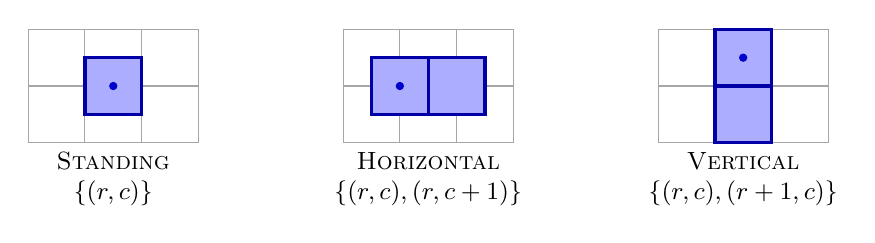
\begin{tikzpicture}[font=\small,
    cell/.style={draw=gray!70, minimum width=0.72cm, minimum height=0.72cm},
    occupied/.style={cell, fill=blue!32, very thick, draw=blue!65!black}]
    \begin{scope}[xshift=0cm]
        \foreach \x in {0,1,2} \foreach \y in {0,1} {
            \node[cell] at (0.72*\x,0.72*\y) {};
        }
        \node[occupied] at (0.72,0.36) {};
        \fill[blue!80!black] (0.72,0.36) circle (1.5pt);
        \node[align=center] at (0.72,-0.82) {\textsc{Standing}\\$\{(r,c)\}$};
    \end{scope}
    \begin{scope}[xshift=4cm]
        \foreach \x in {0,1,2} \foreach \y in {0,1} {
            \node[cell] at (0.72*\x,0.72*\y) {};
        }
        \node[occupied] at (0.36,0.36) {};
        \node[occupied] at (1.08,0.36) {};
        \fill[blue!80!black] (0.36,0.36) circle (1.5pt);
        \node[align=center] at (0.72,-0.82) {\textsc{Horizontal}\\$\{(r,c),(r,c+1)\}$};
    \end{scope}
    \begin{scope}[xshift=8cm]
        \foreach \x in {0,1,2} \foreach \y in {0,1} {
            \node[cell] at (0.72*\x,0.72*\y) {};
        }
        \node[occupied] at (0.72,0.72) {};
        \node[occupied] at (0.72,0) {};
        \fill[blue!80!black] (0.72,0.72) circle (1.5pt);
        \node[align=center] at (0.72,-0.82) {\textsc{Vertical}\\$\{(r,c),(r+1,c)\}$};
    \end{scope}
\end{tikzpicture}
\caption{Ba tư thế của khối nhìn từ trên xuống; chấm đậm là ô mốc}
\label{fig:orientations}
\end{figure}

Hình~\ref{fig:orientations} cho thấy chỉ lưu tọa độ là chưa đủ: cùng một ô mốc
nhưng tư thế khác nhau sẽ chiếm các ô khác nhau, dẫn đến tập hành động hợp
lệ và trạng thái kế tiếp khác nhau.

\subsubsection{Khối tách và mặt nạ trạng thái cầu}

Trong bước xử lý Split Switch, thành phần khối trước hết trở thành
\begin{equation}
b=\operatorname{Split}(p_a,p_b,i),\qquad i\in\{0,1\},
\end{equation}
trong đó $p_a,p_b$ là vị trí hai khối lập phương đơn vị và $i$ xác định khối
đang được điều khiển. Chỉ khối này di chuyển; hành động \textsc{SwitchCube}
đổi $i$ thành $1-i$ mà không đổi vị trí.

Với $k$ cầu, bit thứ $j$ của $m$ cho biết cầu $j$ đang mở hay đóng:
\begin{equation}
\operatorname{Open}(j,m)=((m\mathbin{\gg}j)\mathbin{\&}1)=1.
\end{equation}
Hai trạng thái có cùng vị trí và tư thế nhưng khác mặt nạ cầu là hai đỉnh
khác nhau, vì một nước đi có thể hợp lệ ở trạng thái này nhưng làm khối rơi ở
trạng thái kia. Tương tự, hai trạng thái khối tách chỉ khác khối đang điều
khiển cũng phải được phân biệt.

\subsection{Hành động và chuyển trạng thái}

Tập hành động là
\begin{equation}
A=\{\textsc{Up},\textsc{Down},\textsc{Left},\textsc{Right},
\textsc{SwitchCube}\}.
\end{equation}
Bốn hành động di chuyển áp dụng cho cả hai dạng khối; \textsc{SwitchCube} chỉ
hợp lệ khi khối đã tách. Với khối nguyên, hàm lăn phụ thuộc vào ô mốc hiện tại
$p=(r,c)$, tư thế và hành động. Mỗi ô của Bảng~\ref{tab:orientation-transition}
cho cặp $(p',o')$ sau khi lăn: $p'$ là ô mốc mới, còn $o'$ nhận một trong ba
giá trị $S$ (Standing), $H$ (Horizontal) hoặc $V$ (Vertical).

\begin{table}[H]
\centering
\caption{Ô mốc và tư thế sau khi lăn khối nguyên}
\label{tab:orientation-transition}
\normalsize
\setlength{\tabcolsep}{8pt}
\renewcommand{\arraystretch}{1.25}
\begin{tabular}{@{}lcccc@{}}
\toprule
\textbf{Tư thế trước} & \textbf{Up} & \textbf{Down} & \textbf{Left} & \textbf{Right} \\
\midrule
Standing & $(r-2,c),V$ & $(r+1,c),V$ & $(r,c-2),H$ & $(r,c+1),H$ \\
Horizontal & $(r-1,c),H$ & $(r+1,c),H$ & $(r,c-1),S$ & $(r,c+2),S$ \\
Vertical & $(r-1,c),S$ & $(r+2,c),S$ & $(r,c-1),V$ & $(r,c+1),V$ \\
\bottomrule
\end{tabular}
\end{table}

Khi khối tách, một hành động di chuyển cộng vectơ $(-1,0)$, $(1,0)$,
$(0,-1)$ hoặc $(0,1)$ vào vị trí khối đang được điều khiển. Khối này không
được đi vào vị trí của khối còn lại; một khối lập phương riêng lẻ cũng không
được đi vào Goal. Hai khối tự động ghép khi khoảng cách Manhattan giữa chúng
bằng 1. Nếu kề theo hàng, khối mới có tư thế Horizontal và ô mốc là ô bên
trái; nếu kề theo cột, tư thế là Vertical và ô mốc là ô phía trên.

Hàm chuyển trạng thái được viết dưới dạng
\begin{equation}
T:S\times A\rightarrow S\cup\{\textsc{Invalid},\textsc{Fall}\}.
\end{equation}
Hàm $T$ gồm biến đổi hình học, kiểm tra điều kiện nâng đỡ, kích hoạt công tắc
mới được nhấn, cập nhật trạng thái cầu và kiểm tra lại điều kiện nâng đỡ ở
trạng thái cuối. Một nước đi rơi vào ô không được nâng đỡ không thể kích hoạt
công tắc để ``cứu'' chính nó. Riêng \textsc{SwitchCube} chỉ đổi khối đang điều
khiển, không thay đổi bàn chơi hay kích hoạt lại công tắc.

\subsection{Điều kiện hợp lệ và các cơ chế nâng cao}

\subsubsection{Điều kiện nâng đỡ, Fragile và Goal}

Một chuyển động chỉ hợp lệ khi mọi ô mà khối chiếm đều nằm trong bàn chơi và
được nâng đỡ. Floor, Start và Goal có thể nâng đỡ khối; ô Void chỉ nâng đỡ
được nếu có cầu đang mở. Khối nguyên đứng trên Fragile sẽ rơi, trong khi khối
nằm hoặc khối lập phương riêng lẻ vẫn được nâng đỡ.

\begin{table}[H]
\centering
\caption{Điều kiện nâng đỡ theo loại ô và dạng khối}
\label{tab:support-rules}
\small
\begin{tabular}{@{}lccc@{}}
\toprule
\textbf{Loại ô} & \textbf{Khối đứng} & \textbf{Khối nằm} & \textbf{Khối đơn vị} \\
\midrule
Floor/Start & Hợp lệ & Hợp lệ & Hợp lệ \\
Void hoặc cầu đóng & Rơi & Rơi & Rơi \\
Cầu mở & Hợp lệ & Hợp lệ & Hợp lệ \\
Fragile & Rơi & Hợp lệ & Hợp lệ \\
Goal & Có thể thắng & Được nâng đỡ, chưa thắng & Không được đi vào \\
\bottomrule
\end{tabular}
\end{table}

\subsubsection{Công tắc và cầu}

Công tắc chỉ phát sinh hiệu ứng khi chuyển từ trạng thái chưa bị nhấn sang bị
nhấn. Soft Switch được kích hoạt khi bất kỳ phần nào của khối nguyên hoặc một
khối lập phương đè lên nó. Heavy Switch và Split Switch chỉ được kích hoạt khi
khối nguyên đứng đúng trên công tắc.

Mỗi công tắc có thể tác động tới một hoặc nhiều cầu bằng ba phép toán:
\textsc{Toggle}, \textsc{SetOpen} và \textsc{SetClosed}. Nếu nhiều hiệu ứng cùng
tác động một cầu trong một bước chuyển, \texttt{GameEngine} xử lý số lần
\textsc{Toggle} theo tính chẵn lẻ, sau đó áp dụng \textsc{SetClosed} và cuối
cùng là \textsc{SetOpen}. Vì vậy, \textsc{SetOpen} được ưu tiên khi các hiệu
ứng xung đột. Mặt nạ cầu mới trở thành một phần của trạng thái kế tiếp.

\begin{table}[H]
\centering
\caption{Điều kiện kích hoạt các loại công tắc}
\label{tab:switch-rules}
\small
\begin{tabular}{@{}lcccl@{}}
\toprule
\textbf{Công tắc} & \textbf{Khối đứng} & \textbf{Khối nằm} & \textbf{Khối đơn vị} & \textbf{Tác động chính} \\
\midrule
Soft & Có & Có & Có & Thay đổi trạng thái cầu \\
Heavy & Có & Không & Không & Thay đổi trạng thái cầu \\
Split & Có & Không & Không & Tách và dịch chuyển \\
\bottomrule
\end{tabular}
\end{table}

\subsubsection{Tách và ghép khối}

Split Switch tách khối và đưa hai khối đơn vị tới các vị trí
\texttt{split\_targets}; khối A được điều khiển trước. Mỗi khối đơn vị có thể
kích hoạt Soft Switch nhưng không kích hoạt Heavy/Split Switch hoặc hoàn thành
màn chơi. Nếu hai vị trí đích kề trực giao, \texttt{GameEngine} ghép khối ngay
trong hành động dịch chuyển tức thời. Trường hợp còn lại, người chơi có thể
di chuyển hoặc đổi khối đang điều khiển để đưa hai khối tới vị trí kề nhau.

\begin{figure}[H]
\centering
\resizebox{0.98\textwidth}{!}{%
\begin{tikzpicture}[
    box/.style={draw, rounded corners, fill=blue!8, minimum height=1.1cm,
        text width=3.0cm, align=center},
    flow/.style={-{Latex[length=2.2mm]}, thick}]
    \node[box] (normal) {\texttt{NormalBlock} đứng trên Split Switch};
    \node[box, right=0.7cm of normal] (teleport) {Dịch chuyển tới $p_a,p_b$\\điều khiển khối $A$};
    \node[box, right=0.7cm of teleport] (control) {Di chuyển khối đang điều khiển\\hoặc \textsc{SwitchCube}};
    \node[box, right=0.7cm of control] (adjacent) {$\lVert p_a-p_b\rVert_1=1$};
    \node[box, right=0.7cm of adjacent] (merged) {\texttt{NormalBlock}\\Horizontal\\hoặc Vertical};
    \draw[flow] (normal) -- node[above, font=\footnotesize] {tách} (teleport);
    \draw[flow] (teleport) -- (control);
    \draw[flow] (teleport.north) to[out=65,in=115,looseness=1.2]
        node[above, font=\footnotesize] {hai vị trí đích kề nhau} (adjacent.north);
    \draw[flow] (control) edge[loop below] node[below, font=\footnotesize] {tiếp tục} (control);
    \draw[flow] (control) -- (adjacent);
    \draw[flow] (adjacent) -- node[above, font=\footnotesize] {ghép} (merged);
\end{tikzpicture}%
}
\caption{Vòng đời của khối khi kích hoạt Split Switch và ghép lại}
\label{fig:split-merge}
\end{figure}

\subsection{Trạng thái ban đầu và điều kiện đích}

Trạng thái đầu là $s_0=(\operatorname{Normal}(p_0,\textsc{Standing}),m_0)$,
trong đó $m_0$ mã hóa các cầu mở ban đầu. Tập đích là
\begin{equation}
G=\{(b,m)\in S\mid b=\operatorname{Normal}(g,\textsc{Standing})\}.
\end{equation}
Nói cách khác, khối đang nằm trên Goal hoặc một khối đơn vị ở gần Goal đều không thỏa
điều kiện kết thúc. Từ đây, $g$ luôn là tọa độ ô Goal, còn $G$ là tập các
trạng thái đích.

\subsection{Mô hình tìm kiếm trên đồ thị và hàm chi phí}

Ký hiệu $\mathcal{G}=(V,E)$ dành riêng cho đồ thị tìm kiếm, phân biệt với tập
đích $G$. Tập $V$ gồm các trạng thái hợp lệ có thể đạt từ trạng thái đầu; tập
cạnh được xác định bởi
\begin{equation}
E=\{(s,a,s')\mid T(s,a)=s',\;a\in A\}.
\end{equation}
Chỉ bước chuyển hợp lệ hoặc thắng mới tạo cạnh cho bộ giải; hành động không
hợp lệ và trạng thái rơi bị loại. Nếu $N=R\cdot C$ và có $k$ cầu, một cận trên
đơn giản của số trạng thái là
\begin{equation}
|V|\leq 2^k\left(3N+2N(N-1)\right),
\end{equation}
gồm tối đa $3N$ cấu hình khối nguyên và $2N(N-1)$ cấu hình hai khối đơn vị có
phân biệt khối đang điều khiển. Các điều kiện nâng đỡ và hình học làm số trạng
thái thực tế nhỏ hơn nhiều, nhưng cận này cho thấy mặt nạ cầu và trạng thái
khối tách làm không gian tìm kiếm tăng nhanh.

Đồ thị có chu trình do lăn ngược, đổi trạng thái cầu và đổi khối điều khiển hai
lần. Mỗi đỉnh phải chứa đầy đủ $b$ và $m$ để phân biệt các nước đi tiếp theo.
Vì vậy, các thuật toán cần kiểm soát trạng thái lặp khi tìm kiếm trên đồ
thị~\cite{russell2021}.

Hàm chi phí chuẩn $c:S\times A\times S\rightarrow\{0,1,2\}$ gán trọng số
cho mỗi cạnh hợp lệ như Bảng~\ref{tab:cost}. Chi phí một đường đi là tổng chi
phí các cạnh; các thuật toán khác nhau có thể tối ưu những mục tiêu khác nhau.

\begin{table}[H]
\centering
\caption{Hàm chi phí chuẩn dùng cho UCS và A*}
\label{tab:cost}
\small
\begin{tabular}{@{}llc@{}}
\toprule
\textbf{Hành động} & \textbf{Trường hợp} & \textbf{Chi phí} \\
\midrule
\textsc{SwitchCube} & Chỉ đổi khối đang điều khiển & 0 \\
Di chuyển & Kích hoạt Split Switch; trạng thái sau gồm hai khối đơn vị & 1 \\
Di chuyển & Trạng thái sau chạm Fragile, ngoài trường hợp trên & 2 \\
Di chuyển & Trường hợp hợp lệ còn lại & 1 \\
\bottomrule
\end{tabular}
\end{table}

Với khối nguyên, Fragile được xét ở các ô khối chiếm trong trạng thái sau;
với khối đơn vị đang di chuyển, xét ô đích của khối ấy, kể cả trước khi ghép.
Hành động kích hoạt Split Switch và kết thúc với hai khối đơn vị có chi phí 1,
ngay cả khi một vị trí đích sau dịch chuyển là Fragile. Chi phí của
\textsc{SwitchCube} bằng 0 vì hành động này không đổi vị trí. Quy tắc chi phí
chỉ mô hình hóa mức rủi ro của Fragile, không thay đổi tính hợp lệ của nước đi.

Gọi $\pi=(a_1,\ldots,a_n)$ là lời giải. Số hành động là $n$, gồm cả
\textsc{SwitchCube}; \texttt{solution\_length} chỉ đếm các hành động di chuyển;
\texttt{solution\_cost} là $\sum_j c(s_{j-1},a_j,s_j)$ đối với UCS/A*, còn
BFS/DFS gán mỗi hành động chi phí đơn vị. Do đó, lời giải ít hành động nhất
chưa chắc có ít lần di chuyển nhất hoặc có chi phí chuẩn thấp nhất.

Tóm lại, bài toán tìm kiếm được xác định bởi
\begin{equation}
P=(S,A,T,s_0,G,c),
\end{equation}
với $S$ là tập trạng thái hợp lệ, $A$ là tập hành động, $T$ là quy tắc chuyển,
$s_0$ là trạng thái đầu, $G$ là tập đích và $c$ là hàm chi phí chuẩn. Các chương
sau cho thấy từng thành phần này được hiện thực và khai thác như thế nào.
